\documentclass[conference]{IEEEtran}
\IEEEoverridecommandlockouts
\usepackage{cite}
\usepackage{amsmath,amssymb,amsfonts}
\usepackage{graphicx}
\usepackage{booktabs}
\usepackage{url}
\usepackage{xcolor}
\usepackage[hidelinks]{hyperref}
\graphicspath{{../outputs/}}

% ---- change these two lines once the repository is public ----
\newcommand{\repourl}{https://github.com/Vish-Overflows/cf-skill-dimensions}
\newcommand{\dataurl}{\repourl/releases}
% --------------------------------------------------------------

\begin{document}

\title{Is One Number Enough?\\Searching for Hidden Skill Dimensions in Codeforces Ratings}

\author{\IEEEauthorblockN{Vishnu Sinha}
\IEEEauthorblockA{CS 328 \\ }
\and
\IEEEauthorblockN{Bhavay Goyal}
\IEEEauthorblockA{CS 328 \\ }}

\maketitle

\begin{abstract}
Codeforces summarises every contestant by a single Elo-style rating, which implicitly assumes that competitive-programming skill is one-dimensional. We test this assumption on 589 rated rounds (36{,}519 users, 3{,}773 problems, 15.8\,M user--problem outcomes) from the public Codeforces API. For every outcome we subtract the Elo-expected solve probability and keep the \emph{surprise}; the resulting sparse matrix is analysed with truncated SVD against two null models (within-problem permutation and a parametric Elo simulation), held-out prediction, split-half reliability, rating-band re-analysis, problem clustering against the setters' tags, and MinHash-LSH search for ``skill twins''. The data reject one-dimensionality: the leading singular values exceed every null copy, a rank-10 model predicts held-out solves better than Elo plus user/problem biases (log-loss $0.2045\!\to\!0.1970$, AUC $0.9731\!\to\!0.9749$), and about six user dimensions reproduce across disjoint halves of the rounds (canonical correlations $0.90$--$0.60$ vs.\ $0.03$ under shuffling). The dominant hidden dimension beyond rating is how a user does on easy versus hard problems; the most robust \emph{topical} dimension contrasts mathematics/constructive problems with data-structure/DP/graph problems and survives in every rating band. The official tags, however, align only weakly with data-driven clusters (best-match Jaccard within 1--2 points of random partitions) and ``being good at tag $t$ beyond rating'' is a stable trait only for the algorithmic tags ($r{=}0.19$--$0.27$) and not for sortings, brute force or geometry ($r{\le}0.05$). Skill-twin search with MinHash LSH reaches recall@10 of 0.84 while examining 1.4\,\% of the 641\,M user pairs.
\end{abstract}

\begin{IEEEkeywords}
competitive programming, rating systems, SVD, permutation tests, item response theory, clustering, MinHash, locality-sensitive hashing
\end{IEEEkeywords}

%=====================================================================
\section{Problem Description}
Take two Codeforces users, both rated 1600. One breezes through number theory but freezes on dynamic programming; the other is the exact opposite. As far as Codeforces is concerned they are the same contestant: every user's ability is compressed into one Elo-style rating. The rating carries a strong hidden assumption---that skill is one-dimensional, so if user $A$ is likelier than user $B$ to solve one problem of a given difficulty, the same holds for every other problem of that difficulty.

The assumption matters. Millions of users pick practice problems by rating, recommendation tools filter by rating, and recruiters screen by it. The only other description of a problem is its list of \emph{tags} (\texttt{dp}, \texttt{greedy}, \texttt{math}, \texttt{graphs}, \dots), assigned by hand by problem setters. Neither description has been tested against the data: does either capture how people actually differ?

\textbf{Research question.} Once rating is accounted for, is there any \emph{consistent} structure left in who solves what? If there is, (i) what are the hidden skill dimensions, (ii) do they coincide with the official tags, and (iii) who are a user's ``skill twins''---the users with the most similar pattern of over- and under-performance, regardless of rating? The question is designed so that it can fail: if the residual signal is indistinguishable from noise, ``one number is enough'' is itself the reportable answer.

%=====================================================================
\section{Solution Approach}

\subsection{Survey of Existing Methods}
\textbf{Rating systems.} Elo~\cite{elo} models the probability that one player beats another as a logistic function of the rating difference. Glicko~\cite{glicko} and TrueSkill~\cite{trueskill} add uncertainty; Elo-MMR~\cite{elommr} extends the idea to massive multi-player rounds and is the basis of Codeforces' current system. All of them maintain a \emph{scalar} skill per player. Codeforces additionally assigns each problem a difficulty rating---the rating at which the Elo model predicts a 50\,\% solve probability---estimated from in-contest results.

\textbf{Item response theory.} In psychometrics the same logistic model is the one-parameter (Rasch) model~\cite{rasch}: examinee ability and item difficulty on one latent scale. Multidimensional IRT~\cite{mirt} relaxes this to a vector of abilities and a vector of item loadings; our analysis is a non-parametric version of asking ``how many dimensions does the Codeforces item pool need?''

\textbf{Low-rank residual analysis and significance.} Matrix factorisation of user--item matrices is the standard tool in recommender systems~\cite{koren}. Deciding how many components are real is classically done by parallel analysis~\cite{horn}---compare eigenvalues against those of random data with the same marginals---and permutation tests for PCA~\cite{buja}. We follow this tradition, with a within-column shuffle that keeps each problem's distribution and sparsity pattern.

\textbf{Educational data mining.} Knowledge tracing~\cite{bkt,dkt} and $Q$-matrix/DINA models~\cite{dina} represent a learner by a vector of skill masteries and each item by the skills it requires. The Codeforces tag list is, in effect, a hand-made $Q$-matrix; part of our question is whether the data support it.

\textbf{Similarity search.} MinHash~\cite{broder} estimates Jaccard similarity of sets from short signatures, and banding the signatures gives a locality-sensitive hashing scheme~\cite{indyk,mmds} whose candidate threshold is approximately $(1/b)^{1/r}$ for $b$ bands of $r$ rows.

\subsection{Data}
Everything comes from the public Codeforces API (no scraping): \texttt{problemset.problems} for each problem's difficulty rating and tags, \texttt{contest.standings} for which official contestant solved which problem during the round, and \texttt{contest.ratingChanges} for each participant's rating \emph{before} the round. We selected the 600 most recent finished individual rounds (Div.~1--4, Educational and Global rounds; Codeforces Round~706 to Round~1116) that were at least 90 days old so that problem ratings had settled; 11 turned out to be unrated and were dropped, leaving 589 rounds. We kept users with at least 40 rated participations in this sample: 36{,}519 of 455{,}111 rated participants (median 57 rounds; median last rating 1420, IQR 1228--1623, maximum 3792). Only team rounds, virtual and out-of-competition rows are excluded. The pull took 1{,}187 API calls at the required one call per two seconds and is cached to disk.

\subsection{The Surprise Matrix}
For user $i$ with pre-contest rating $R_i$ and problem $j$ with difficulty $r_j$, the Elo expected solve probability is
\begin{equation}
p_{ij} = \frac{1}{1 + 10^{(r_j - R_i)/400}}.
\end{equation}
With $y_{ij}=1$ if the user solved the problem in-contest and $0$ otherwise, the \emph{surprise} is $s_{ij} = y_{ij} - p_{ij}$: positive for solving something hard, negative for missing something easy. Rating is thereby subtracted out. Pairs the user never faced are $0$ (``no evidence''), giving a sparse $36{,}519\times3{,}773$ matrix $S$ with $15{,}848{,}852$ observed entries (density $0.115$). The mean observed surprise is $+0.029$ (Elo is slightly pessimistic for these regular competitors), the standard deviation $0.259$, and $39.1\,\%$ of observed pairs were solved. Because $y\in\{0,1\}$, both $y$ and $p$ are recoverable from $s$, which we exploit for the parametric null and the held-out evaluation.

\subsection{Hidden Axes: Truncated SVD and Two Null Models}
We compute a truncated SVD $S\approx U\Sigma V^{\top}$ (\texttt{scipy.sparse.linalg.svds}, $k{=}20$ and $k{=}60$). \emph{Null 1 (permutation):} shuffle the observed surprises within each problem's column---every problem keeps its own surprise distribution and exactly the same set of observing users, but any user-level consistency is destroyed---recompute the spectrum, repeat 20 times (10 for $k{=}60$). Component $k$ is called significant if $\sigma_k$ exceeds the $k$-th singular value of \emph{every} shuffled copy. \emph{Null 2 (parametric):} keep the mask and the Elo probabilities, redraw $y_{ij}\sim\mathrm{Bernoulli}(p_{ij})$, i.e.\ simulate the world in which rating is the whole story, 10 times. We also repeat Null~1 after subtracting each user's mean surprise in each round, which removes ``good day / bad day'' and form effects shared by all problems of a round.

Each surviving axis is read off its highest- and lowest-loading problems and their tags; for every tag we compute an enrichment $z$-score (mean loading of tagged versus untagged problems) and, to separate topic from difficulty, the correlation of the loadings with problem rating.

\subsection{Does the Structure Generalise? Held-out Prediction}
Significance against a shuffle shows the structure is not noise; it does not show it is \emph{useful}. We therefore split the observed entries $80/10/10$ into train, calibration and test. The SVD is fitted on train only; a three-parameter logistic calibration (features: $\operatorname{logit}p_{ij}$, additive user/problem biases fitted on train, and the rank-$k$ reconstruction $\hat s_{ij}$) is fitted on the calibration split; log-loss, Brier score and AUC are reported on test. Two hold-out designs are used: random cells, and whole (user, round) blocks so that the model cannot lean on the user's other results in the same round.

\subsection{Is It a Trait? Split-half Reliability}
We split the rounds into odd and even halves, fit a $k{=}10$ SVD on each half separately, and compute canonical correlations between users' axis-score matrices $U_A\Sigma_A$ and $U_B\Sigma_B$, against a null where the users of one half are permuted. We also compute, for each tag, every user's mean surprise on problems carrying that tag (minus the user's overall mean) in each half and correlate across halves: is ``good at \texttt{dp} beyond rating'' a stable trait?

\subsection{Within-band Analysis}
Because only strong users face Div.~1 problems, zero-filling can manufacture axes that merely encode ``which division you compete in''. We repeat the SVD and permutation test inside three bands of mean user rating (1000--1400, 1400--1800, 1800--2400), keeping problems observed by at least 300 band users.

\subsection{Grouping Problems and Comparing with Tags}
Each problem receives coordinates $V\Sigma$ on the significant axes (standardised). We cluster with $k$-means ($k$ by silhouette, and a sweep $k{=}2..12$) and with spectral clustering on a 15-nearest-neighbour graph. Treating each cluster and each tag as a set of problems, agreement is the mean over clusters of the best-match Jaccard similarity, compared with 200 random partitions of the same cluster sizes. As a complementary, less partition-sensitive measure we ask whether a problem's tag can be predicted from its axis coordinates: five-fold cross-validated AUC of logistic regression using (a) rating only, (b) the 20 axis coordinates only, (c) both, and (b) with shuffled labels.

\subsection{Skill Twins with MinHash LSH}
Each user becomes a set of tokens: \texttt{hit:}$j$ for problems solved with $p_{ij}<0.3$ and \texttt{miss:}$j$ for problems missed with $p_{ij}>0.7$. Two users are skill twins if these sets have high Jaccard similarity. All-pairs comparison of 35{,}811 users is 641\,M pairs, so we compute 256 MinHash signatures per user with the universal hash family $h(x)=(ax+b)\bmod(2^{31}{-}1)$, band them into $b\times r$ blocks, and verify candidate pairs with exact Jaccard. On a 3{,}000-user sample we compute exact top-10 neighbours by brute force and report recall@10, candidate fraction and wall-clock speed-up for several $(b,r)$; the chosen setting is then run on the full population against a chunked exact baseline. A command-line demo and a Streamlit app take a handle and return the user's score on each axis next to their rating, plus their top twins.

%=====================================================================
\section{Results}

\subsection{There Is Structure Beyond Rating (D1)}
\begin{figure}[t]
\centering
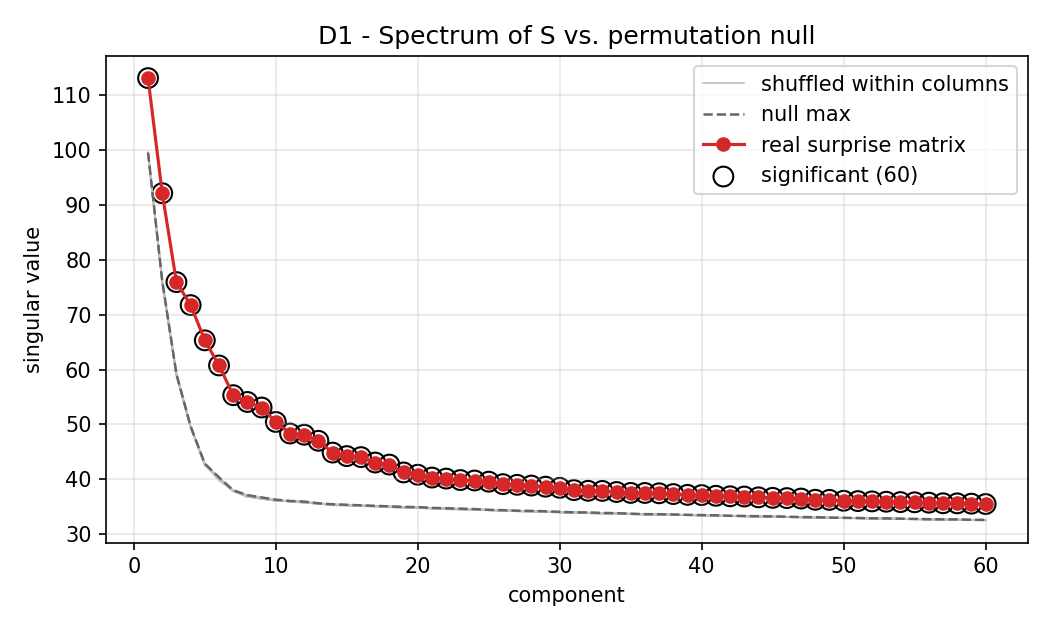
\includegraphics[width=\columnwidth]{D1_spectrum_k60.png}
\caption{Singular values of the real surprise matrix ($k{=}60$) against ten within-column permutations. Every component clears the null maximum; the gap is widest for components 4--9.}
\label{fig:d1}
\end{figure}
\begin{figure}[t]
\centering
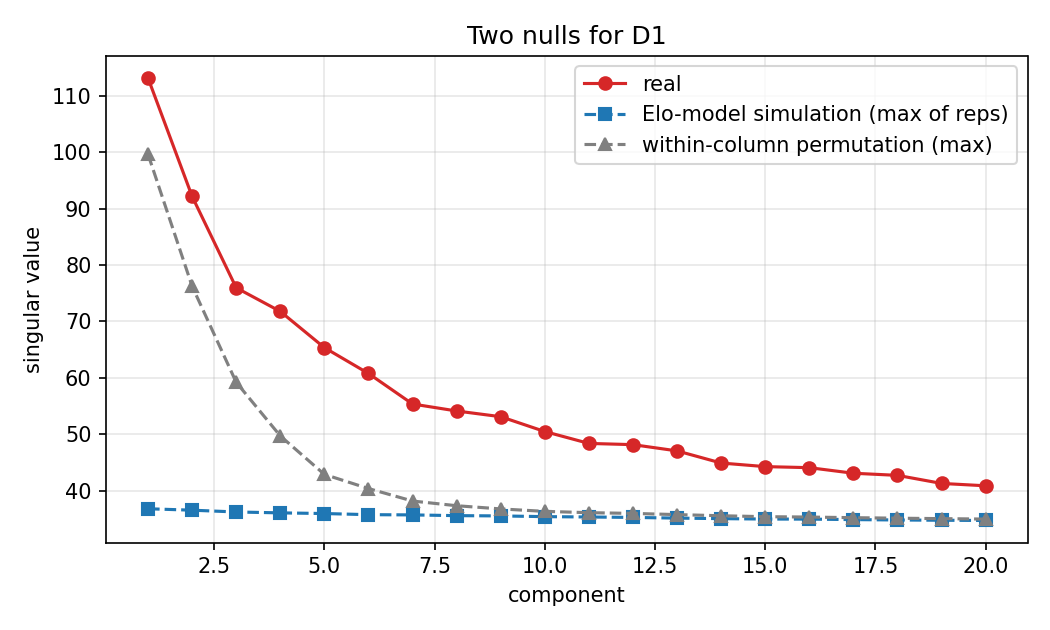
\includegraphics[width=\columnwidth]{R_paramnull.png}
\caption{Two nulls for the first 20 components: within-column permutation and parametric Elo simulation ($y_{ij}\sim\mathrm{Bernoulli}(p_{ij})$). The real spectrum is far above both.}
\label{fig:paramnull}
\end{figure}

Fig.~\ref{fig:d1} and Table~\ref{tab:d1} show the spectrum against the permutation null. All 60 tested components exceed every shuffled copy; the ratio $\sigma_k/\max_{\text{null}}\sigma_k$ rises from $1.14$ at $k{=}1$ to $1.52$ at $k{=}5$ and decays slowly to $1.09$ at $k{=}60$. Against the parametric Elo null (Fig.~\ref{fig:paramnull}) the separation is larger still---$3.08\times$, $2.52\times$, $2.10\times$ for the first three components---because a Bernoulli world has no user-level correlation at all. Subtracting each user's per-round mean does not remove the structure: ratios become $1.24, 1.34, 1.49, 1.65, 1.67, 1.66,\dots$ for the first six components.

\begin{table}[t]
\caption{Spectrum versus within-column permutation null (\texttt{D1\_spectrum\_k60.csv}).}
\label{tab:d1}
\centering
\begin{tabular}{rrrr}
\toprule
component & $\sigma$ (real) & $\sigma$ (null max) & ratio \\
\midrule
1 & 113.1 & 99.6 & 1.14 \\
2 & 92.2 & 76.2 & 1.21 \\
3 & 76.0 & 59.2 & 1.28 \\
4 & 71.8 & 49.7 & 1.44 \\
5 & 65.3 & 42.9 & \textbf{1.52} \\
6 & 60.8 & 40.4 & 1.51 \\
7--9 & 55.3--53.1 & 38.0--36.7 & 1.46 \\
10 & 50.5 & 36.3 & 1.39 \\
20 & 40.8 & 34.9 & 1.17 \\
60 & 35.5 & 32.6 & 1.09 \\
\bottomrule
\end{tabular}
\end{table}

With $15.8$\,M observations the test is extremely powerful, so ``60 significant components'' must not be read as ``60 skills''. The effect-size evidence below locates the useful content in roughly the first ten.

\subsection{The Structure Predicts Unseen Solves}
\begin{figure*}[t]
\centering
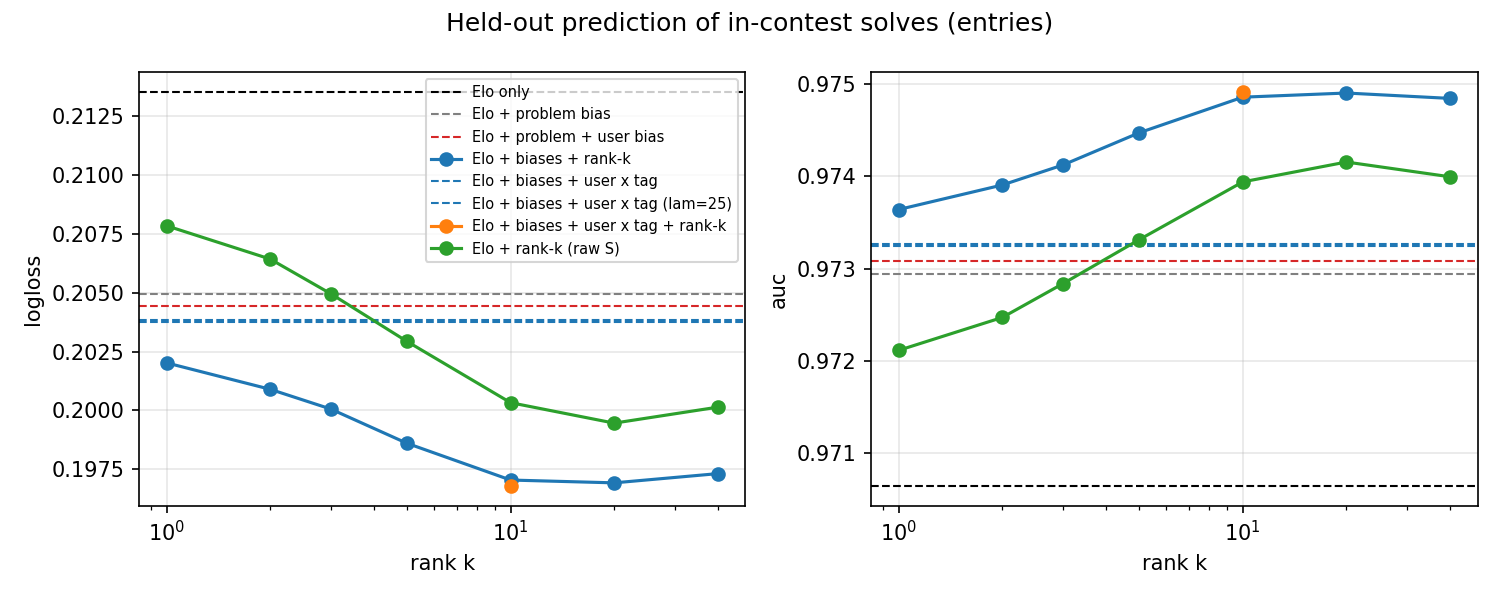
\includegraphics[width=0.9\textwidth]{R_heldout_entries.png}
\caption{Held-out prediction of 1.59\,M hidden in-contest outcomes (random cells). Dashed lines: Elo only; Elo + problem bias; Elo + problem + user bias. Curves: rank-$k$ reconstruction added to the bias model (blue) or to raw Elo (orange). Gains peak at $k{=}10$--$20$ and reverse at $k{=}40$.}
\label{fig:heldout}
\end{figure*}

Table~\ref{tab:heldout} and Fig.~\ref{fig:heldout} report the held-out evaluation. Elo alone has log-loss $0.2135$ and AUC $0.9706$---the rating is already a very good predictor. Adding a per-problem bias (i.e.\ allowing the problem's official rating to be mis-calibrated) gives the single largest gain ($0.2050$); a per-user bias adds almost nothing ($0.2045$). On top of both, a rank-10 reconstruction lowers log-loss to $0.1970$ and raises AUC to $0.9749$, a $3.7\,\%$ relative gain beyond the bias model and $7.7\,\%$ beyond Elo. The gain saturates at $k{=}20$ and reverses at $k{=}40$ (over-fitting), which is consistent with the ratio curve in Table~\ref{tab:d1}. Hiding whole (user, round) blocks gives the same picture (best $k{=}10$, log-loss $0.2144\!\to\!0.1987$), so the gain does not come from leakage within a round. Interestingly, in that design the user bias coefficient drops to $0.84$ (from $6.2$): a user's average form does not carry across rounds nearly as well as the low-rank structure does.

\begin{table}[t]
\caption{Held-out prediction, random-cell split (\texttt{R\_heldout\_entries.csv}). Relative gain is in log-loss vs.\ Elo only.}
\label{tab:heldout}
\centering
\begin{tabular}{lrrrr}
\toprule
model & $k$ & log-loss & AUC & gain \\
\midrule
Elo only & -- & 0.2135 & 0.9706 & -- \\
+ problem bias & -- & 0.2050 & 0.9729 & 4.0\,\% \\
+ problem + user bias & -- & 0.2045 & 0.9731 & 4.2\,\% \\
+ biases + rank-$k$ & 1 & 0.2020 & 0.9736 & 5.4\,\% \\
 & 5 & 0.1986 & 0.9745 & 7.0\,\% \\
 & \textbf{10} & \textbf{0.1970} & \textbf{0.9749} & \textbf{7.7\,\%} \\
 & 20 & 0.1969 & 0.9749 & 7.8\,\% \\
 & 40 & 0.1973 & 0.9748 & 7.6\,\% \\
Elo + rank-$k$ (raw $S$) & 20 & 0.1995 & 0.9742 & 6.6\,\% \\
\midrule
\multicolumn{5}{l}{\emph{whole (user, round) blocks hidden}} \\
Elo only & -- & 0.2144 & 0.9705 & -- \\
+ biases & -- & 0.2055 & 0.9728 & 4.2\,\% \\
+ biases + rank-$k$ & 10 & 0.1987 & 0.9745 & 7.3\,\% \\
\bottomrule
\end{tabular}
\end{table}

\subsection{The Dimensions Are Stable Traits}
\begin{figure*}[t]
\centering
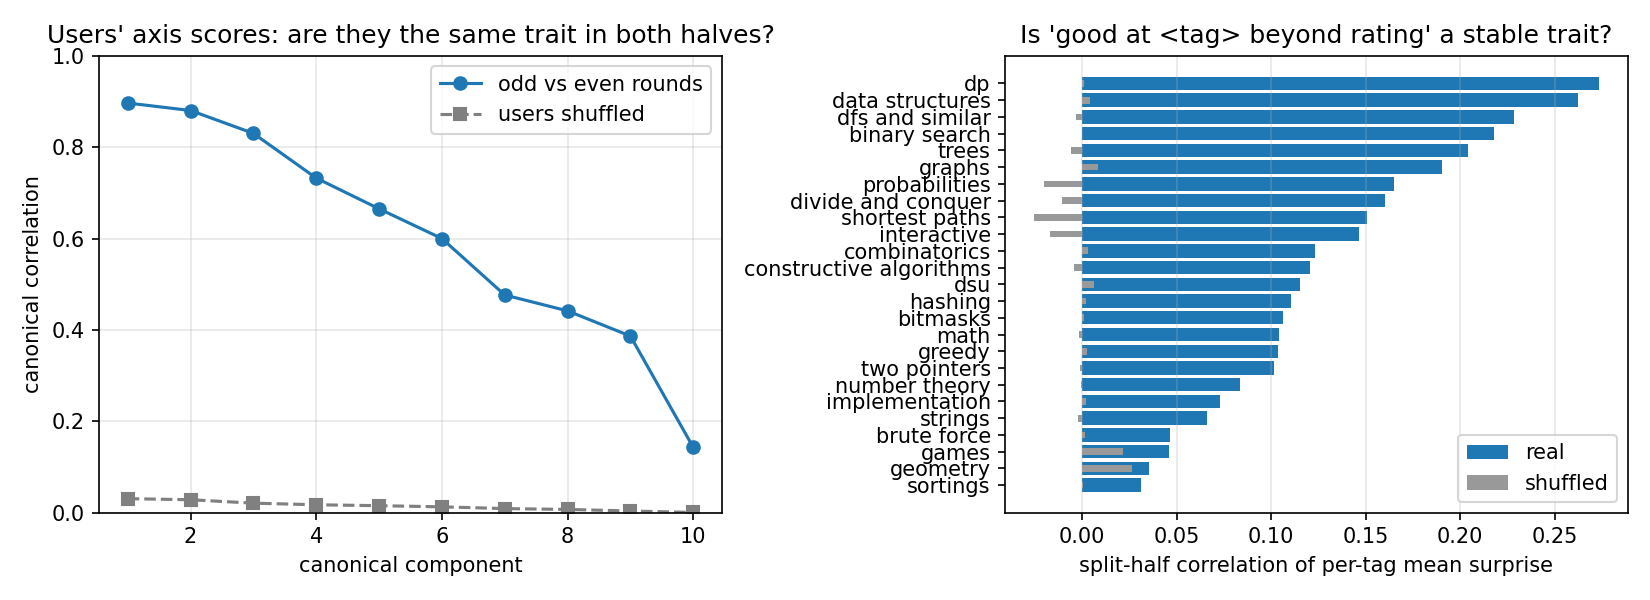
\includegraphics[width=0.95\textwidth]{R_splithalf.png}
\caption{Split-half reliability (odd vs.\ even rounds). Left: canonical correlations between users' ten axis scores in the two halves (blue) and after permuting users (grey). Right: split-half correlation of each user's mean surprise on problems with a given tag, after removing the user's overall mean.}
\label{fig:splithalf}
\end{figure*}

Fitting the SVD separately on odd and even rounds (Fig.~\ref{fig:splithalf}, left) gives canonical correlations of $0.90, 0.88, 0.83, 0.73, 0.67, 0.60, 0.48, 0.44, 0.39, 0.14$ between the two halves' user scores, against $\le 0.03$ when users are shuffled. Roughly six user dimensions are reproducible from independent sets of problems. The first axis alone correlates $0.82$ across halves.

At the level of tags (Fig.~\ref{fig:splithalf}, right), being systematically above or below one's Elo expectation on a tag is a stable trait for the algorithmic tags---\texttt{dp} $r{=}0.27$, \texttt{data structures} $0.26$, \texttt{dfs and similar} $0.23$, \texttt{binary search} $0.22$, \texttt{trees} $0.20$, \texttt{graphs} $0.19$---and only weakly so for \texttt{math} and \texttt{greedy} ($0.10$), \texttt{implementation} ($0.07$), and essentially not at all for \texttt{brute force}, \texttt{games}, \texttt{geometry} and \texttt{sortings} ($0.03$--$0.05$). Shuffled controls are all within $\pm0.03$.

\subsection{What the Hidden Dimensions Are (D2)}
Table~\ref{tab:axes} summarises the leading axes. Three patterns recur.

\begin{table*}[t]
\caption{Leading skill axes: tag enrichment at each end ($z$-scores in parentheses), correlation of problem loadings with problem rating, and mean rating of the 15 most extreme problems at each end (\texttt{D2\_axes.md}). Signs are arbitrary.}
\label{tab:axes}
\centering
\footnotesize
\begin{tabular}{@{}clp{5.2cm}p{5.6cm}rrr@{}}
\toprule
axis & $\sigma$ & enriched at ``$+$'' end & enriched at ``$-$'' end & $\rho$(load., rating) & rating$_+$ & rating$_-$ \\
\midrule
1 & 113 & implementation (+5.8), strings (+4.2), greedy (+3.4) & dfs ($-$22.6), trees ($-$21.4), divide \& conquer ($-$20.9), dp ($-$19.8) & $-0.47$ & 840 & 1200 \\
2 & 92 & implementation (+2.4), combinatorics (+2.1), data structures (+2.0) & constructive ($-$3.1), greedy ($-$2.3), math ($-$2.2) & $0.01$ & 800 & 913 \\
3 & 76 & dp (+6.7), combinatorics (+5.4), trees (+5.3), graphs (+4.9) & math ($-$0.7), games, strings & $0.14$ & 1040 & 833 \\
4 & 72 & greedy (+9.0), constructive (+3.4), binary search (+2.8) & meet-in-the-middle ($-$8.9), suffix structures ($-$8.8), trees ($-$7.0), fft ($-$6.7) & $-0.17$ & 1327 & 840 \\
5 & 65 & meet-in-the-middle (+5.7), probabilities (+5.5), graphs (+4.1) & greedy ($-$3.4), games ($-$2.1), math ($-$1.8) & $0.09$ & 913 & 1160 \\
8 & 54 & math (+7.6), constructive (+4.6), geometry (+2.5), number theory (+1.9) & data structures ($-$8.4), trees ($-$6.1), binary search ($-$6.1), dfs ($-$5.7) & $-0.11$ & 1220 & 1240 \\
11 & 48 & dp (+4.2), data structures (+3.9), binary search (+3.5) & constructive ($-$5.1), games ($-$4.0), greedy ($-$1.6) & $0.00$ & 1313 & 1033 \\
12 & 48 & constructive (+4.9), greedy (+3.9) & combinatorics ($-$4.9), binary search ($-$4.7), math ($-$4.5), dp ($-$3.4) & $-0.05$ & 1167 & 1187 \\
\bottomrule
\end{tabular}
\end{table*}

\textbf{Axis 1 is ``solving above or below your weight''.} Its positive end is the easy Div.~3/4 \texttt{A}--\texttt{B} problems (mean rating 840; \texttt{implementation}, \texttt{strings}) and its negative end hard graph/DP/tree problems (mean rating 1200); loadings correlate $-0.47$ with problem rating. Users at the negative end over-perform on hard algorithmic problems relative to their rating (tourist and jiangly sit at the 12th--13th percentile); users at the positive end reliably clean up easy problems but do not reach further. This is real structure beyond rating, but it is closer to a difficulty-slope or under-rating effect than to a topic, and in the within-band analysis its ratio falls to $1.00$--$1.06$, confirming that much of it is a between-division effect.

\textbf{The robust topical dimension is ad-hoc versus algorithmic.} Constructive / greedy / math / number theory / geometry on one side and dp / data structures / trees / graphs / binary search on the other appears on axes 2, 3, 4, 8, 11 and 12 with low rating correlation ($|\rho|\le0.17$; axis~8 has both ends rated $\approx 1230$). The same contrast is the clearest topical axis inside every rating band: axis~7 of the 1000--1400 band (math, number theory, constructive vs.\ trees, data structures, dfs; $\rho{=}-0.17$), axes~4--5 of the 1400--1800 band (math, constructive, geometry vs.\ data structures, dp, dfs; $\rho{=}-0.11$), and axis~5 of the 1800--2400 band (math, number theory, combinatorics vs.\ dfs, data structures, trees; $\rho{=}-0.05$). It also survives per-round residualisation (axis~2 of the residualised run: combinatorics, dp, data structures vs.\ constructive).

\textbf{A heavy-algorithms pool axis.} Meet-in-the-middle, suffix structures, fft, flows and probabilities versus greedy/implementation (axes 4--6, 9--10) partly reflects which users ever face such problems, i.e.\ a Div.~1 pool effect of zero-filling.

\subsection{Tags Capture the Dimensions Only Weakly (D3)}
\begin{figure}[t]
\centering
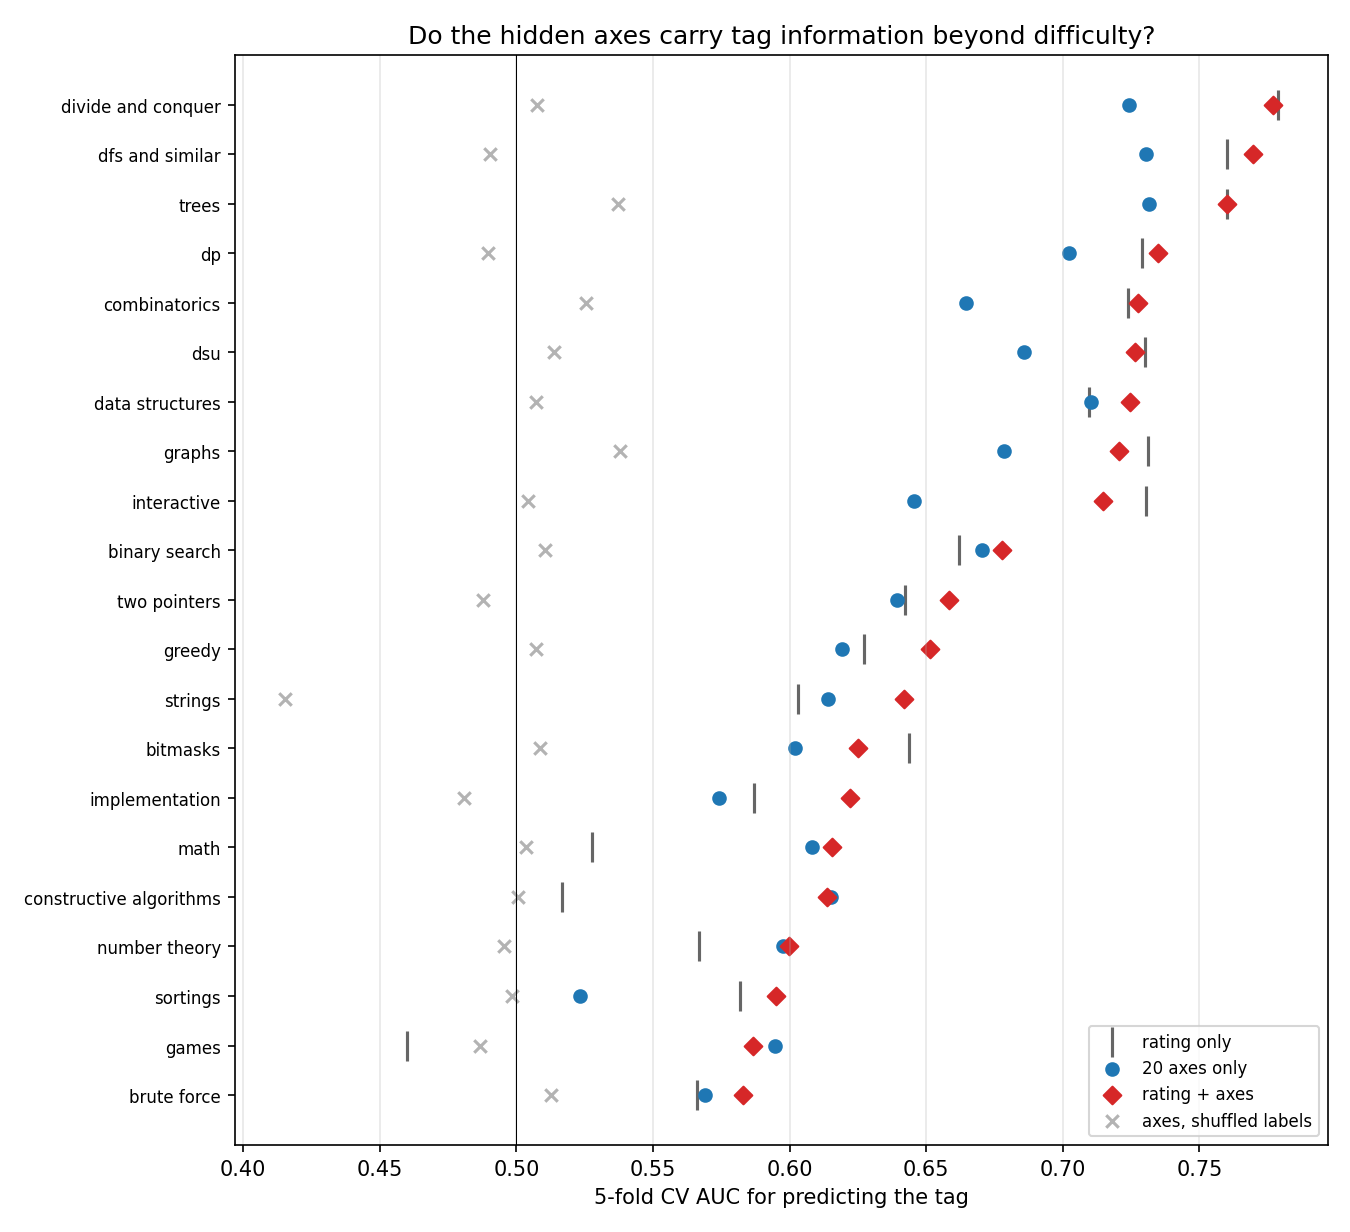
\includegraphics[width=\columnwidth]{R_tagpred.png}
\caption{Five-fold cross-validated AUC for predicting each tag from problem rating alone, from the 20 axis coordinates alone, from both, and from the axes with shuffled labels.}
\label{fig:tagpred}
\end{figure}

Restricting to the 3{,}326 problems observed by at least 1{,}000 users, $k$-means with $k{=}8$ on the 20 significant axes attains a mean best-match Jaccard of $0.097$ against $0.094\pm0.001$ for random partitions of the same sizes ($z{=}2.5$, $p{=}0.015$); spectral clustering attains $0.131$ against $0.108$ ($z{=}17.7$). Across the sweep $k{=}2..12$ the agreement is $0.000$--$0.010$ above random. The difference is statistically reliable but the effect is tiny, and the clusters that are found are organised by difficulty and division rather than topic: for $k{=}8$ one cluster holds 2{,}130 problems of mean rating 2035 and the other seven are 800--1400-rated Div.~3/4 problems split by their position in the round. The residualised axes give the same picture ($0.103$ vs.\ $0.099$; spectral $0.123$ vs.\ $0.118$).

The predictive view (Fig.~\ref{fig:tagpred}) is more nuanced. Difficulty alone predicts many tags well---\texttt{dp} AUC $0.73$, \texttt{trees} $0.76$---simply because hard problems are tagged with hard techniques. The axes add information beyond difficulty mainly for the ad-hoc tags: \texttt{math} $0.53\!\to\!0.62$, \texttt{constructive algorithms} $0.52\!\to\!0.61$, \texttt{games} $0.46\!\to\!0.59$, \texttt{number theory} $0.57\!\to\!0.60$, \texttt{strings} $0.60\!\to\!0.64$, \texttt{implementation} $0.59\!\to\!0.62$, \texttt{greedy} $0.63\!\to\!0.65$---and essentially nothing for \texttt{dp}, \texttt{trees}, \texttt{graphs} or \texttt{data structures}, whose tag information is already carried by rating. Shuffled-label controls are at $0.50\pm0.04$. Tags are therefore \emph{related} to the hidden dimensions, but they do not partition problems the way users' behaviour does.

\subsection{Skill Twins and LSH Evaluation (D4, D5)}
\begin{figure}[t]
\centering
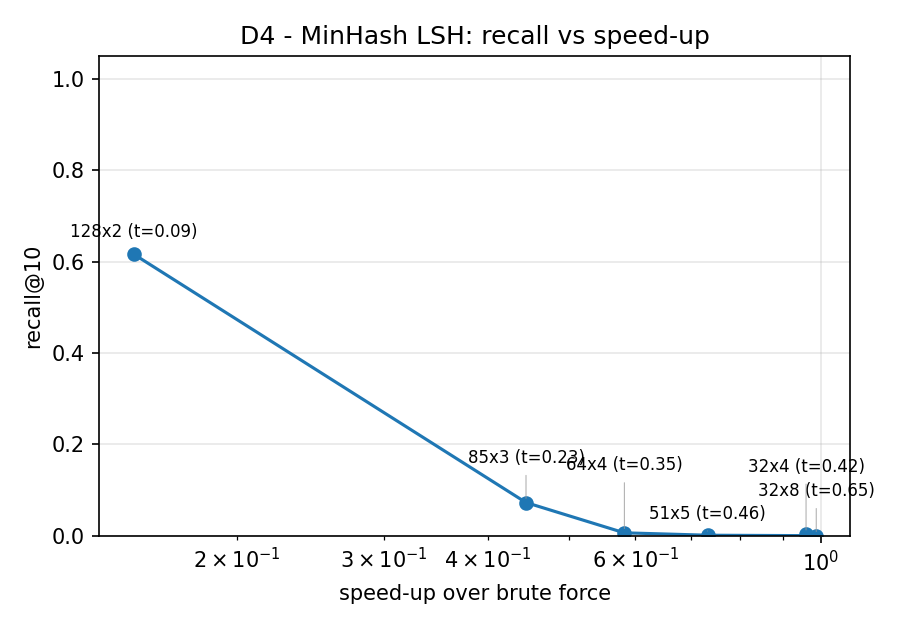
\includegraphics[width=\columnwidth]{D4_lsh_eval.png}
\caption{MinHash LSH on a 3{,}000-user sample: recall@10 against exact neighbours versus wall-clock speed-up for several band/row settings (256 hashes).}
\label{fig:d4}
\end{figure}

With the $|s_{ij}|>0.7$ token rule, 35{,}811 users have at least five tokens (median 15) over 6{,}025 distinct tokens. A central empirical fact is that \emph{nearest neighbours are far apart}: on the 3{,}000-user sample the exact top-1 Jaccard has median $0.119$ (90th percentile $0.171$) and the tenth neighbour has median $0.071$. The $32\times4$ banding proposed originally (threshold $\approx0.42$) is therefore correct LSH tuned for a similarity level that does not exist in the data and finds essentially nothing (67 candidate pairs, recall $0.003$). Table~\ref{tab:lsh} and Fig.~\ref{fig:d4} report low-threshold settings with 256 hashes.

\begin{table}[t]
\caption{LSH settings on the 3{,}000-user sample (\texttt{D4\_lsh\_eval.csv}) and the full-population run (\texttt{D4\_full\_run.json}).}
\label{tab:lsh}
\centering
\begin{tabular}{rrrrr}
\toprule
$b\times r$ & threshold & cand.\ fraction & recall@10 & speed-up \\
\midrule
$128\times2$ & 0.088 & 1.4\,\% & \textbf{0.617} & 0.13$\times$ \\
$85\times3$ & 0.227 & 0.07\,\% & 0.073 & 0.33$\times$ \\
$64\times4$ & 0.354 & 0.002\,\% & 0.006 & 0.46$\times$ \\
$51\times5$ & 0.455 & $\sim$0 & 0.001 & 0.56$\times$ \\
$32\times8$ & 0.648 & 0 & 0.000 & 0.79$\times$ \\
\midrule
\multicolumn{5}{l}{full population, 35{,}811 users, $128\times2$:} \\
\multicolumn{5}{l}{8.89\,M candidates = 1.39\,\% of 641\,M pairs; recall@10 = \textbf{0.839};} \\
\multicolumn{5}{l}{LSH 42.6\,s vs.\ chunked brute force 11.9\,s (0.28$\times$).} \\
\bottomrule
\end{tabular}
\end{table}

On the full population the $128\times2$ setting examines $1.39\,\%$ of all pairs and recovers $83.9\,\%$ of the exact top-10 neighbours (recall is higher than on the sample because true neighbours are closer when there are more users). The algorithmic saving is real; the wall-clock speed-up is not ($0.28\times$): with sets this small, a sparse matrix product in BLAS already computes all $641$\,M Jaccard values in 12\,s, whereas our Python banding and de-duplication of 8.9\,M candidate pairs costs 43\,s. LSH would win only at a larger $n$ or with a compiled implementation.

The demo (\texttt{python -m cfskills.demo tourist jiangly}) places both top-rated users at the 12th--13th percentile of axis~1 and near the median elsewhere; they are each other's closest twin ($J{=}0.216$), followed by Radewoosh, ksun48, maroonrk, Benq and Um\_nik. Twins are necessarily rating-neighbours, since users can only share tokens on problems they both faced.

%=====================================================================
\section{Conclusions}
\textbf{One number is not enough.} After subtracting the Elo expectation, who solves what is strongly non-random: the leading singular values of the surprise matrix exceed every within-problem shuffle and every Elo simulation, the structure survives removing per-round form, a rank-10 model predicts held-out solves better than Elo plus user and problem biases, and about six user dimensions reproduce across disjoint halves of the rounds. These are four independent tests that could each have said no.

\textbf{But most of the extra information is not ``topics'' in the tag sense.} The largest hidden dimension is how a user does on easy versus hard problems relative to rating---a difficulty slope that also absorbs under-rating and speed. The most robust topical dimension, present in every rating band, contrasts ad-hoc mathematics/constructive problems with data-structure/DP/graph problems; it is a coarse dichotomy rather than a per-tag skill vector. Being ``good at tag $t$ beyond rating'' is a stable trait only for the algorithmic tags.

\textbf{Tags are related to, but do not partition, the hidden structure.} Data-driven clusters match tags only 1--2 Jaccard points better than random partitions, and the axes add predictive information about a tag mainly for the ad-hoc tags whose difficulty does not already reveal them. A single ``algorithmic vs.\ ad-hoc'' label would describe user differences better than the current 35-tag taxonomy.

\textbf{Practical implications.} A rating plus two or three axis scores (difficulty slope, ad-hoc vs.\ algorithmic, heavy-algorithm exposure) would describe a contestant materially better than the rating alone, and problem recommenders could target a user's weak side. For skill-twin search, MinHash LSH is the right tool for the pair-count problem but, at $n\approx36$k with sparse-BLAS available, brute force is faster in practice.

\textbf{Limitations.} Zero-filling unobserved pairs biases the spectrum test towards finding nothing but lets ``which division you compete in'' leak into some axes; the within-band analysis addresses this partially. Problem ratings are themselves estimated from solve data (mild circularity), and a per-problem bias term captures their mis-calibration---the single largest predictive gain we found. Div.~3/4 and Educational rounds are rated only for lower-rated users, so most observations concern 800--1400-rated problems. Only in-contest solves are used, so every surprise is measured under the same time pressure and implementation speed is folded into axis~1. The permutation null destroys all user-level dependence, so with 15.8\,M entries even weak effects are significant; we therefore emphasise effect sizes (singular-value ratios, held-out gains, split-half correlations) over counts of significant components.

%=====================================================================
\section*{Code and Data}
Code (Python; \texttt{cfskills} package with one module per step, 21 unit tests, a Makefile that reproduces every figure and table in this report) is available at \url{\repourl}. The cached raw API pull (115\,MB) and the processed surprise matrix are published as release assets at \url{\dataurl}; alternatively \texttt{make fetch} rebuilds them from the public API in about 75 minutes.

\section*{Contributions}
Vishnu Sinha: API pull, surprise matrix, SVD and null tests, D1--D2. Bhavay Goyal: MinHash LSH, its evaluation, and the demo, D4--D5. Shared: clustering, tag comparison (D3), robustness analyses, and the report.

%=====================================================================
\begin{thebibliography}{00}
\bibitem{elo} A.~E. Elo, \emph{The Rating of Chessplayers, Past and Present}. New York: Arco, 1978.
\bibitem{glicko} M.~E. Glickman, ``Parameter estimation in large dynamic paired comparison experiments,'' \emph{J. Royal Statistical Society C}, vol.~48, no.~3, pp.~377--394, 1999.
\bibitem{trueskill} R.~Herbrich, T.~Minka, and T.~Graepel, ``TrueSkill: A Bayesian skill rating system,'' in \emph{Advances in Neural Information Processing Systems 19}, 2007.
\bibitem{elommr} A.~Ebtekar and P.~Liu, ``Elo-MMR: A rating system for massive multiplayer competitions,'' in \emph{Proc. The Web Conference (WWW)}, 2021.
\bibitem{rasch} G.~Rasch, \emph{Probabilistic Models for Some Intelligence and Attainment Tests}. Copenhagen: Danmarks P{\ae}dagogiske Institut, 1960.
\bibitem{mirt} M.~D. Reckase, \emph{Multidimensional Item Response Theory}. New York: Springer, 2009.
\bibitem{koren} Y.~Koren, R.~Bell, and C.~Volinsky, ``Matrix factorization techniques for recommender systems,'' \emph{IEEE Computer}, vol.~42, no.~8, pp.~30--37, 2009.
\bibitem{horn} J.~L. Horn, ``A rationale and test for the number of factors in factor analysis,'' \emph{Psychometrika}, vol.~30, pp.~179--185, 1965.
\bibitem{buja} A.~Buja and N.~Eyuboglu, ``Remarks on parallel analysis,'' \emph{Multivariate Behavioral Research}, vol.~27, no.~4, pp.~509--540, 1992.
\bibitem{bkt} A.~T. Corbett and J.~R. Anderson, ``Knowledge tracing: Modeling the acquisition of procedural knowledge,'' \emph{User Modeling and User-Adapted Interaction}, vol.~4, pp.~253--278, 1995.
\bibitem{dkt} C.~Piech \emph{et al.}, ``Deep knowledge tracing,'' in \emph{Advances in Neural Information Processing Systems 28}, 2015.
\bibitem{dina} J.~de~la~Torre, ``DINA model and parameter estimation: A didactic,'' \emph{J. Educational and Behavioral Statistics}, vol.~34, no.~1, pp.~115--130, 2009.
\bibitem{broder} A.~Z. Broder, ``On the resemblance and containment of documents,'' in \emph{Proc. Compression and Complexity of Sequences}, 1997, pp.~21--29.
\bibitem{indyk} P.~Indyk and R.~Motwani, ``Approximate nearest neighbors: Towards removing the curse of dimensionality,'' in \emph{Proc. 30th ACM STOC}, 1998, pp.~604--613.
\bibitem{mmds} J.~Leskovec, A.~Rajaraman, and J.~D. Ullman, \emph{Mining of Massive Datasets}, 3rd ed. Cambridge Univ. Press, 2020, ch.~3.
\end{thebibliography}

\end{document}
